

\subsection{SPC evaluation}
\label{sec:eval_spc}
The evaluation section is now shifted to examine the images produced by the SPC. The images will be analyzed using the using a range of methods to examine the performance of the SPC. In this section the BRISQUE algorithm will be used again where connections to the previous result is drawn, a reconstructed image will be compared to an ideal image using homography, a set of images is presented reconstructed at different subsampling ratios, a edge response analysis i performed and the correlation between reconstruction performance and noise is conducted. 



\subsubsection{Image quality using no reference quality assessment}
In this section the blind quality assessment tool BRISQUE will be used to score the reconstructed images from the SPC. The same algorithm was used on the simulated data where a benchmark was set as a theoretical limit to the reconstructed images.\\[0.1in]     

Each image is evaluated at subsampling rate from $5\%$ to $30\%$ where the result is presented in figure~\ref{fig:brisque_plot}.

\begin{figure}[H]
    \centering
    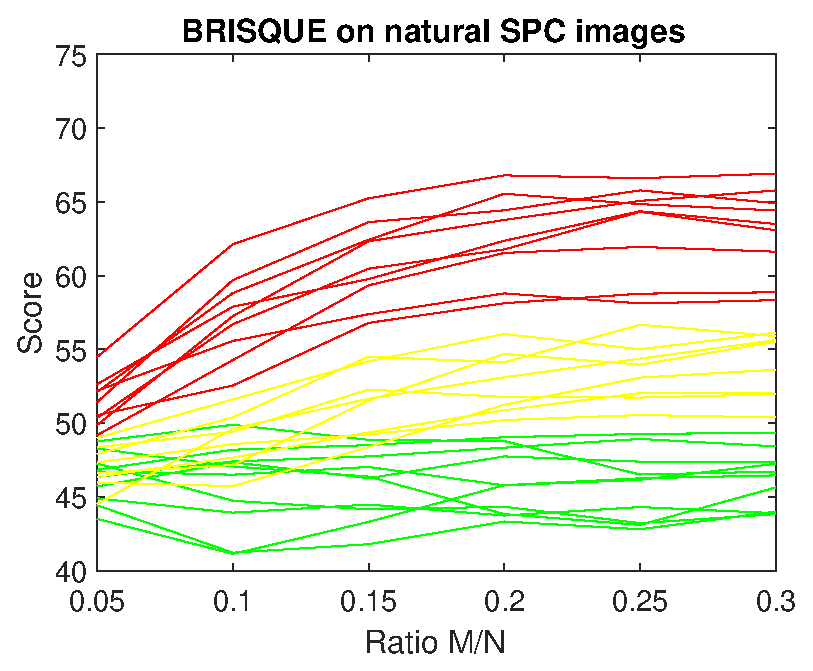
\includegraphics[width = 0.7\linewidth]{result/SPC_NRQA/brisque_spc.eps}
    \caption{BRISQUE score for images reconstructed from the SPC with subsampling ratios from $5\%$ to $30\%$. Each line represent one image and is classified with different colors representing start score at smallest subsampling ratio and general trend when subsampling ratio is increased.}
    \label{fig:brisque_plot}
\end{figure}


As seen in figure~\ref{fig:brisque_plot} each image as been plotted separately, this is because the high variance in the scores and the distinct different trends in the score. Furthermore the images has been classified into three different classes 


\begin{figure}[H]
    \centering
    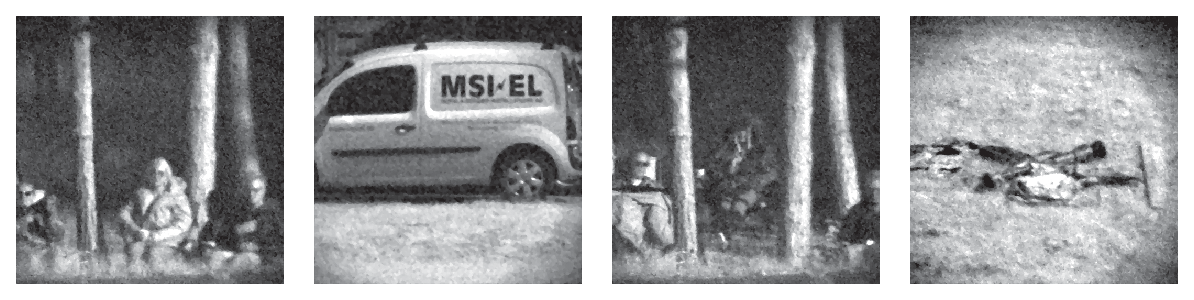
\includegraphics[width = 1\linewidth]{result/SPC_NRQA/good.eps}
    \caption{Example of 'good' images corresponding to the green lines in figure~\ref{fig:brisque_plot}.}
    \label{fig:good_plot}
\end{figure}

\begin{figure}[H]
    \centering
    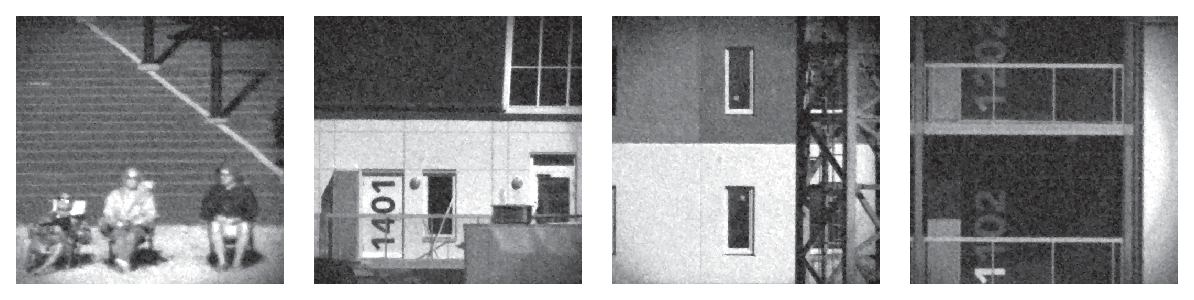
\includegraphics[width = 1\linewidth]{result/SPC_NRQA/half.eps}
    \caption{Example of 'medium good' images corresponding to the yellow lines in figure~\ref{fig:brisque_plot}.}
    \label{fig:half_plot}
\end{figure}

\begin{figure}[H]
    \centering
    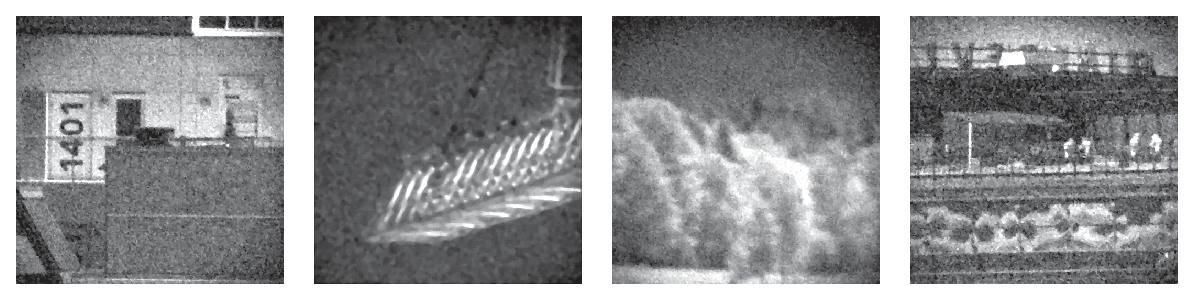
\includegraphics[width = 1\linewidth]{result/SPC_NRQA/bad.eps}
    \caption{Example of 'bad' images corresponding to the red lines in figure~\ref{fig:brisque_plot}.}
    \label{fig:bad_plot}
\end{figure}

\begin{itemize}
    \item Good images are: Strong light, No movement in the image
    \item Medium good images are: Good light, Movement, Brisque bad?
    \item Bad images are: Can have bad light, movement 
\end{itemize}

\subsubsection{Number of measurements}
\begin{figure}[H]
\begin{minipage}[t]{0.3\linewidth} %Car
	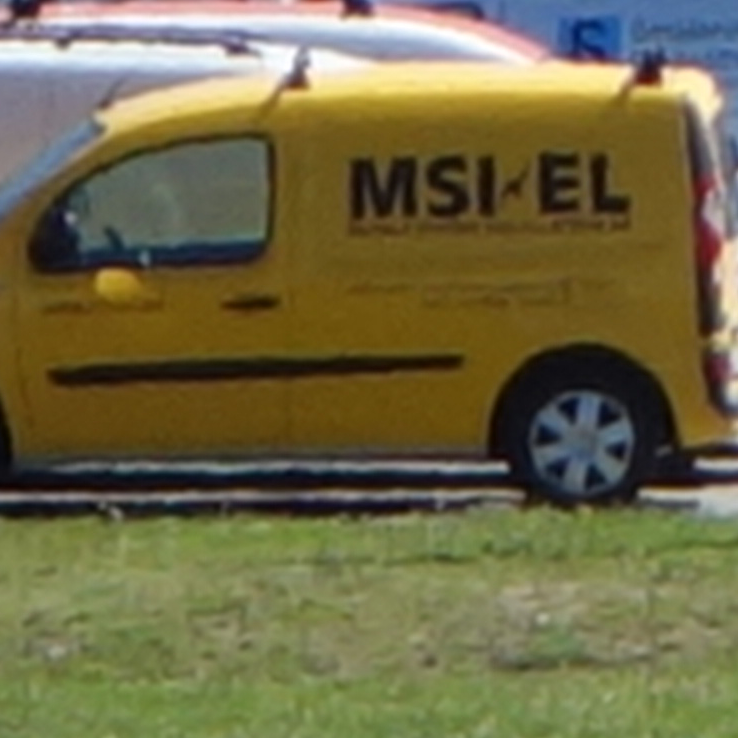
\includegraphics[width = 1\linewidth]{gfx/car/car_org.png}
	\label{fig:car_org}
\end{minipage}
\begin{minipage}[t]{0.3\linewidth} % Hus
	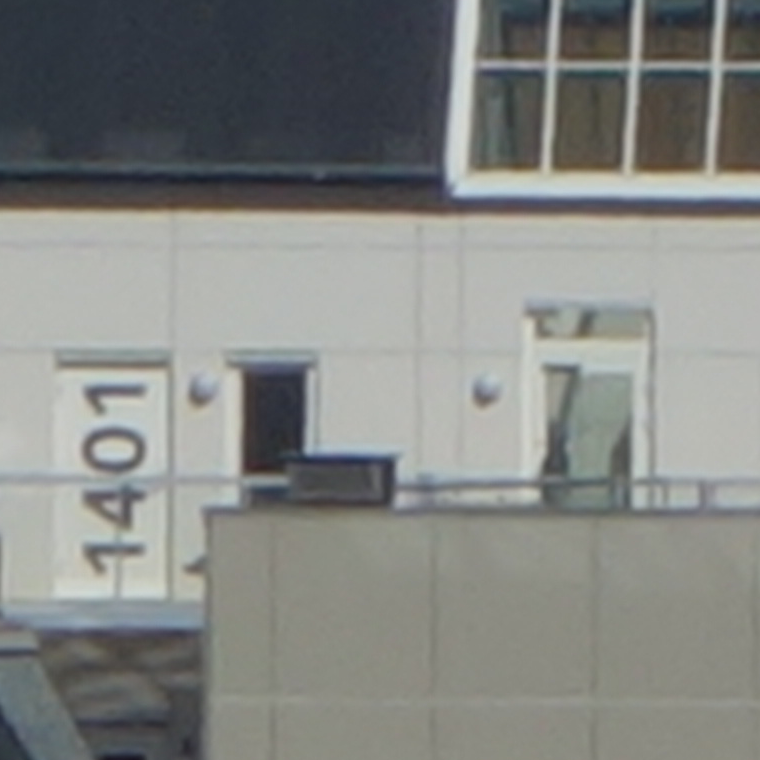
\includegraphics[width = 1\linewidth]{gfx/hus/hus_org.png}
	\label{fig:hus_org}
\end{minipage}
\begin{minipage}[t]{0.3\linewidth} %Sit
	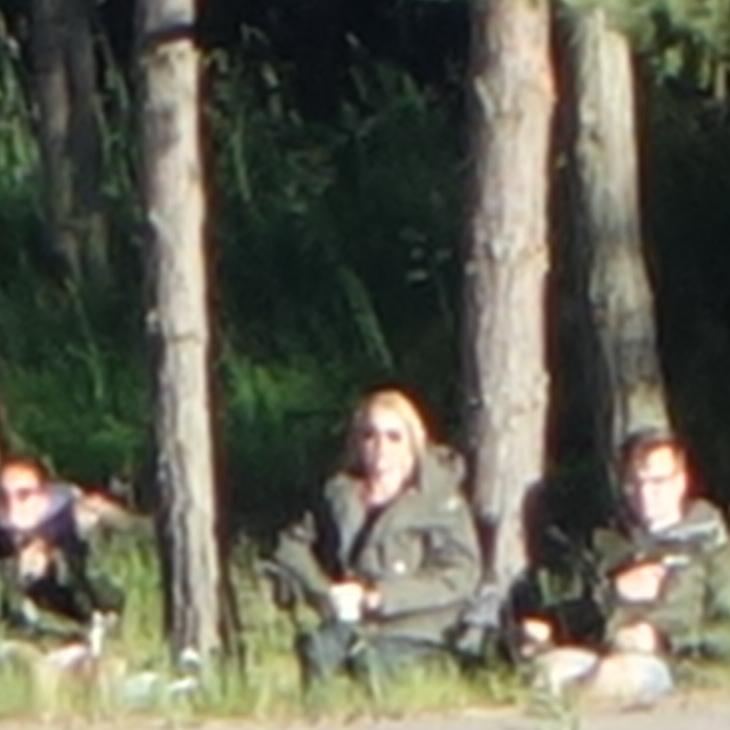
\includegraphics[width = 1\linewidth]{gfx/sit/sit_org.png}
	\label{fig:sit_org}
\end{minipage}
\end{figure}
\begin{figure}[H]
\vspace*{-1.2cm}
\begin{minipage}[t]{0.3\linewidth} %Car
	
\includegraphics[width = 1\linewidth]{gfx/car/car_m5.png}
	\label{fig:car_m5}
\end{minipage}
\begin{minipage}[t]{0.3\linewidth} % Hus
	
\includegraphics[width = 1\linewidth]{gfx/hus/hus_m5.png}
	\label{fig:hus_m5}
\end{minipage}
\begin{minipage}[t]{0.3\linewidth} %Sit
	
\includegraphics[width = 1\linewidth]{gfx/sit/sit_m10.png}
	\label{fig:sit_m5}
\end{minipage}
\end{figure}
\begin{figure}[H]
\vspace*{-1.2cm}
\begin{minipage}[t]{0.3\linewidth} %Car
	
\includegraphics[width = 1\linewidth]{gfx/car/car_m10.png}
	%\subcaption{m15}
	\label{fig:car_m10}
\end{minipage}
\begin{minipage}[t]{0.3\linewidth} % Hus
	
\includegraphics[width = 1\linewidth]{gfx/hus/hus_m10.png}
	%\subcaption{m10}
	\label{fig:hus_m10}
\end{minipage}
\begin{minipage}[t]{0.3\linewidth} %Sit
	
\includegraphics[width = 1\linewidth]{gfx/sit/sit_m10.png}
	%\subcaption{m10}
	\label{fig:sit_m10}
\end{minipage}
\end{figure}
\begin{figure}[H]
\vspace*{-1.2cm}
\begin{minipage}[t]{0.3\linewidth} %Car
	
\includegraphics[width = 1\linewidth]{gfx/car/car_m15.png}
	\subcaption{m15}
	\label{fig:car_m15}
\end{minipage}
\begin{minipage}[t]{0.3\linewidth} % Hus
	
\includegraphics[width = 1\linewidth]{gfx/hus/hus_m15.png}
	\subcaption{m10}
	\label{fig:hus_m15}
\end{minipage}
\begin{minipage}[t]{0.3\linewidth} %Sit
	
\includegraphics[width = 1\linewidth]{gfx/sit/sit_m15.png}
	\subcaption{m10}
	\label{fig:sit_m15}
\end{minipage}
\end{figure}
\begin{figure}[H]
\vspace*{-1.2cm}
\begin{minipage}[t]{0.3\linewidth} %Car
	
\includegraphics[width = 1\linewidth]{gfx/car/car_m20.png}
	%\subcaption{m15}
	\label{fig:car_m20}
\end{minipage}
\begin{minipage}[t]{0.3\linewidth} % Hus
	
\includegraphics[width = 1\linewidth]{gfx/hus/hus_m20.png}
	%\subcaption{m10}
	\label{fig:hus_m20}
\end{minipage}
\begin{minipage}[t]{0.3\linewidth} %Sit
	
\includegraphics[width = 1\linewidth]{gfx/sit/sit_m20.png}
	%\subcaption{m10}
	\label{fig:sit_m20}
\end{minipage}
\end{figure}
\begin{figure}[H]
\begin{minipage}[t]{0.3\linewidth} %Car
	
\includegraphics[width = 1\linewidth]{gfx/car/car_m25.png}
	%\subcaption{m15}
	\label{fig:car_m25}
\end{minipage}
\begin{minipage}[t]{0.3\linewidth} % Hus
	
\includegraphics[width = 1\linewidth]{gfx/hus/hus_m25.png}
	%\subcaption{m10}
	\label{fig:hus_m25}
\end{minipage}
\begin{minipage}[t]{0.3\linewidth} %Sit
	
\includegraphics[width = 1\linewidth]{gfx/sit/sit_m25.png}
	%\subcaption{m20}
	\label{fig:sit_m25}
\end{minipage}
\end{figure}
\begin{figure}[H]
\vspace*{-1.2cm}
\begin{minipage}[t]{0.3\linewidth} %Car
	
\includegraphics[width = 1\linewidth]{gfx/car/car_m30.png}
	%\subcaption{m15}
	\label{fig:car_m30}
\end{minipage}
\begin{minipage}[t]{0.3\linewidth} % Hus
	
\includegraphics[width = 1\linewidth]{gfx/hus/hus_m30.png}
	%\subcaption{m10}
	\label{fig:hus_m30}
\end{minipage}
\begin{minipage}[t]{0.3\linewidth} %Sit
	
\includegraphics[width = 1\linewidth]{gfx/sit/sit_m30.png}
	%\subcaption{m10}
	\label{fig:sit_m30}
\end{minipage}
	\caption{Images reconstructed using $M/N = 5\% \text{ to } 30\%$ measurements from top down.} 
\end{figure}

\subsubsection{Soft chessboard}
\todo[inline]{Todo: Skapa rekonstruerade bilder från homagraphin och jämnför de rekonstruerade med referensbilden}
This evaluation is designed to confirm that the images reconstructed by the SPC follows the same characteristics as the reconstruction of the synthetic data.


\begin{figure}[H]
    \centering
\begin{minipage}[h]{0.3\textwidth}
	\vspace*{1cm}
    
\includegraphics[width=1\textwidth]{result/hom/im_ref.png}
    \subcaption{Refrence image}
    \label{fig:hom_ref}
\end{minipage}
\begin{minipage}[t]{0.22\textwidth}
    
\includegraphics[width = \textwidth]{result/hom/im_m5.png}
    \subcaption{5\%}
    \label{fig:hom_5}
    
\includegraphics[width = \textwidth]{result/hom/im_m20.png}
    \subcaption{20\%}
    \label{fig:hom_20}
\end{minipage}
\begin{minipage}[t]{0.22\textwidth}
    
\includegraphics[width = \textwidth]{result/hom/im_m10.png}
    \subcaption{10\%}
    \label{fig:hom_10}
    
\includegraphics[width = \textwidth]{result/hom/im_m25.png}
    \subcaption{25\%}
    \label{fig:hom_25}
\end{minipage}
\begin{minipage}[t]{0.22\textwidth}
    
\includegraphics[width = \textwidth]{result/hom/im_m15.png}
    \subcaption{15\%}
    \label{fig:hom_15}
    
\includegraphics[width = \textwidth]{result/hom/im_m30.png}
    \subcaption{30\%}
    \label{fig:hom_30}
\end{minipage}

    \caption{The reconstructed images with different number of measurements and the reference image transformed to fit the SPC images using homography.}
    \label{fig:hom_over_im}
\end{figure}


\begin{figure}[H]
    \centering
\begin{minipage}[t]{0.49\textwidth}
    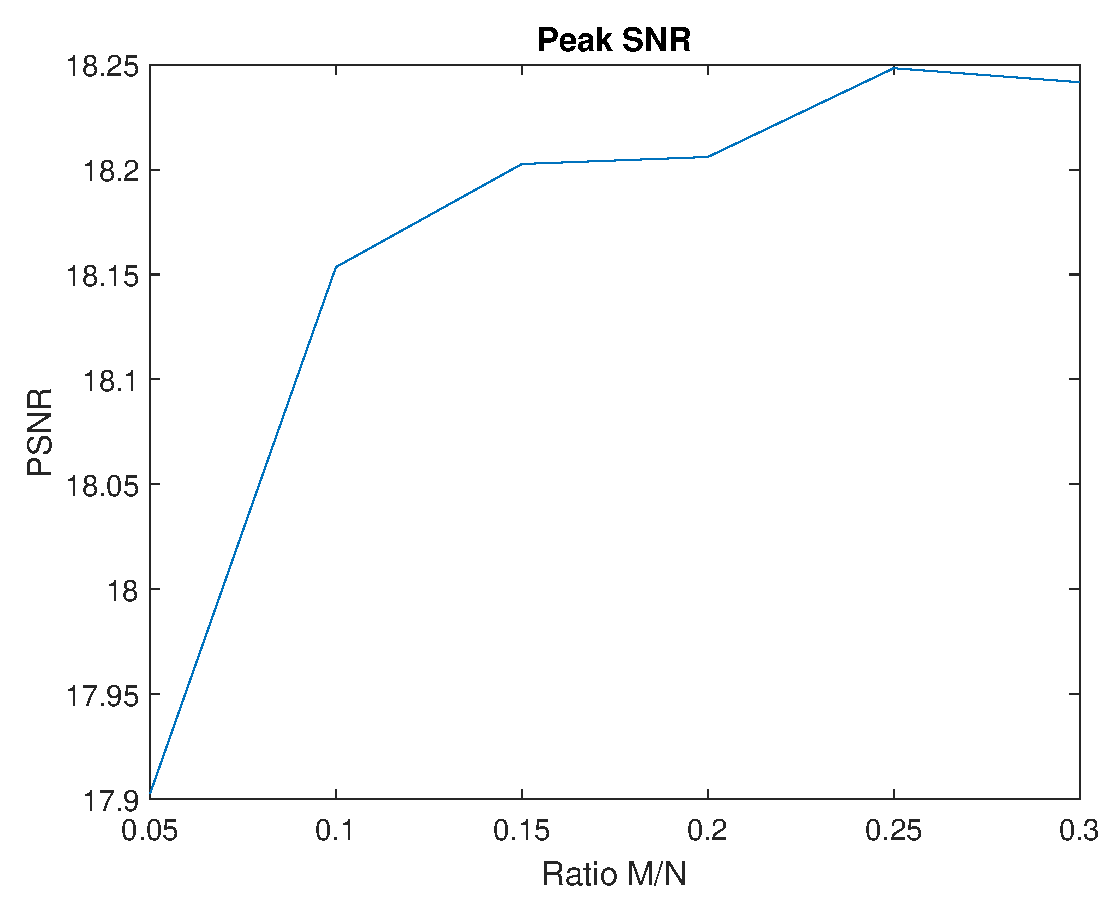
\includegraphics[width=1\textwidth]{result/homo/PSNR_2.eps}
    \subcaption{}
    \label{fig:hom_psnr}
\end{minipage}
\begin{minipage}[t]{0.49\textwidth}
    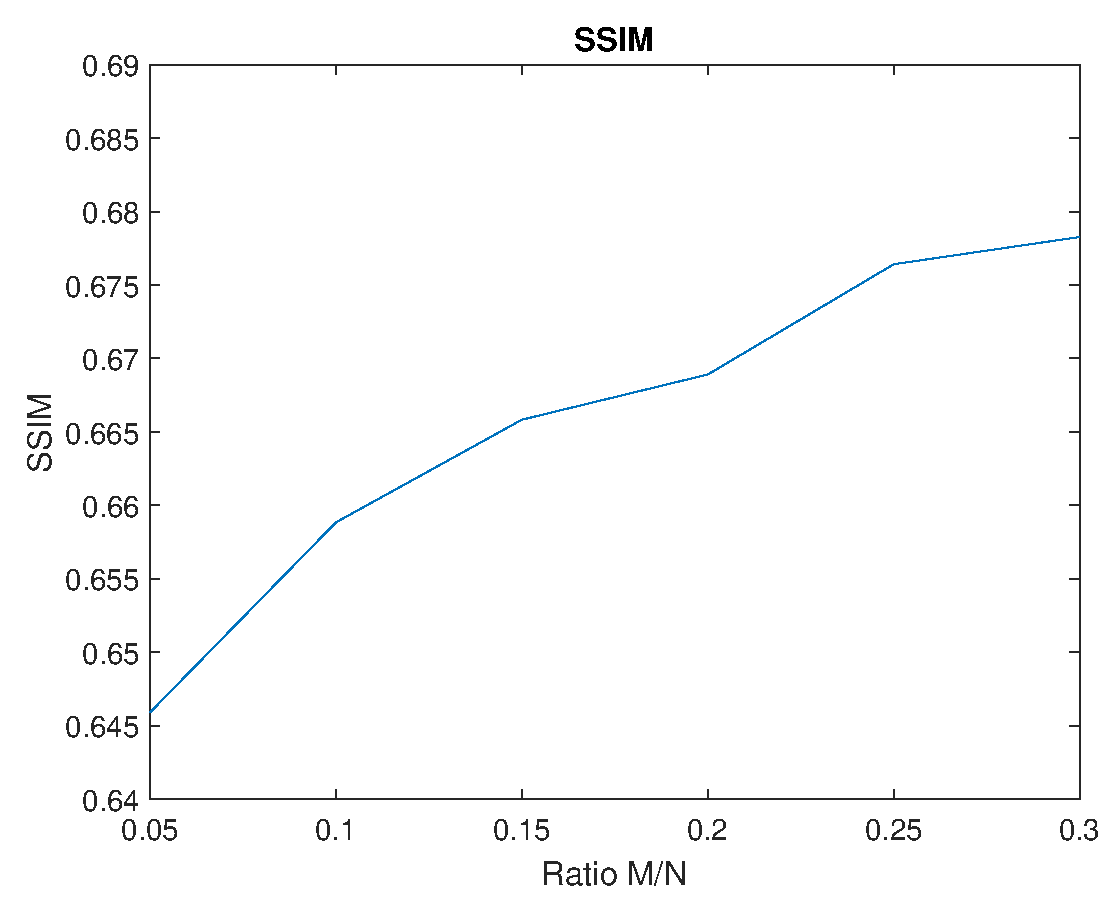
\includegraphics[width=1\textwidth]{result/homo/SSIM_2.eps}
    \subcaption{}
    \label{fig:hom_ssim}
\end{minipage}
    \caption{Signal quality of SPC images compared to reference image. (a) Peak SNR for reconstructed images against reference image. (b) SSIM score for reconstructed images against reference image.}
    \label{fig:hom_score}
\end{figure}





\subsubsection{Modulation Transfer Function}
The MTF is used to comparing the sharpness of cameras and lenses.  

%for two reasons: (1) Image contrast is half its low frequency or peak values,hence detail is still quite visible. The eye is relatively insensitive to detail at spatial frequencies where MTF is low: 10 or less. (2) The response of most cameras falls off rapidly in the vicinity of MTF50 and MTF50P. MTF50P is a better metric for strongly sharpened cameras that have “halos” near edges and corresponding peaks in their MTF response.

The MTF from the SPC is compared to a state of the art SWIR camera. Two scenes was captured by the SPC and a conventional SWIR camera containing printed sheath of paper with simple tilted shapes on them, see figure~\ref{fig:mtf_target}. 



\begin{figure}[H]
    \centering
    
\includegraphics[width=0.9\linewidth]{result/mtf/Target.eps}
    \caption{Printed targets with markings where the MTF measurements was performed}
    \label{fig:mtf_target}
\end{figure}

\begin{figure}[H]
    \centering
\begin{minipage}[t]{0.45\textwidth}
    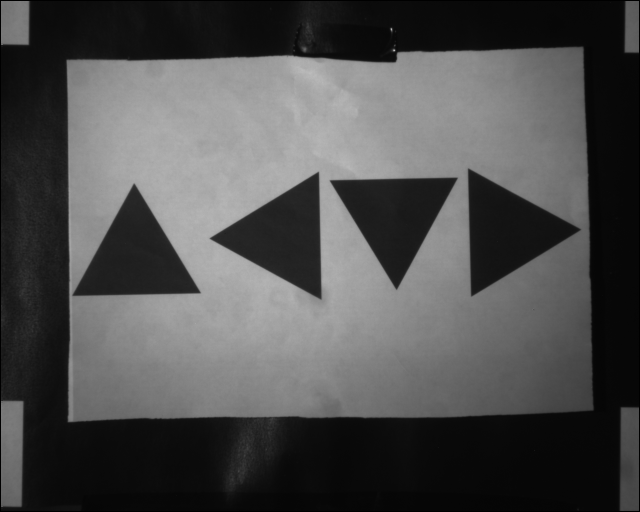
\includegraphics[width=1\textwidth]{result/mtf/swir2.png}
    \subcaption{}
    \label{fig:mtf_s2}
\end{minipage}
\begin{minipage}[t]{0.45\textwidth}
    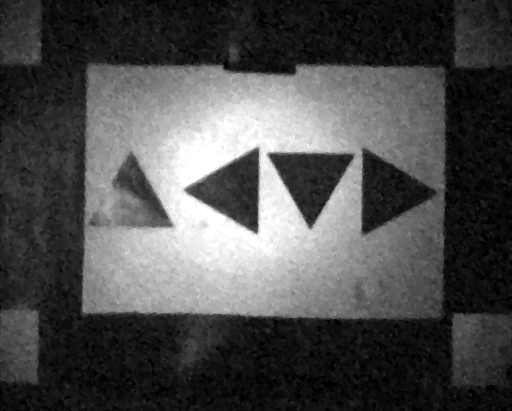
\includegraphics[width=1\textwidth]{result/mtf/spc22.png}
    \subcaption{}
    \label{fig:mtf_spc2}
\end{minipage}
\begin{minipage}[t]{0.45\textwidth}
    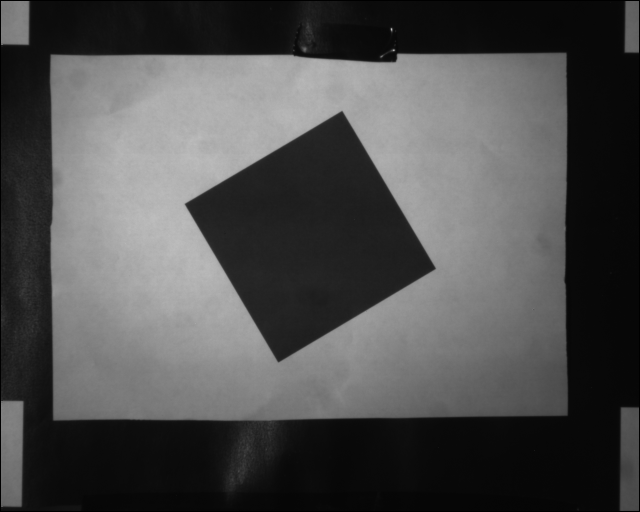
\includegraphics[width=1\textwidth]{result/mtf/swir1.png}
    \subcaption{}
    \label{fig:mtf_s1}
\end{minipage}
\begin{minipage}[t]{0.45\textwidth}
    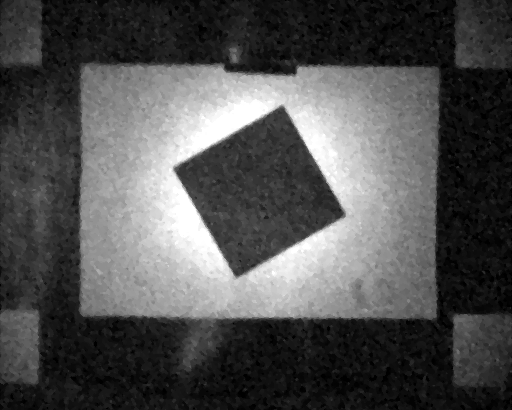
\includegraphics[width=1\textwidth]{result/mtf/spc12.png}
    \subcaption{}
    \label{fig:mtf_spc1}
\end{minipage}
    \caption{SPC and state of the art SWIR camera output images.}
    \label{fig:mtf_target_im}
\end{figure}

In the resulting images MTF measurements was performed on the specified edges to gather a mean and standard deviation for each camera. For the SPC, images reconstructed from 5\% to 30\% was tested in order to see if the number of measurements effected the MTF result. In figure~\ref{fig:mtf_target_im} the images from the SWIR camera and SPC are presented.



\todo[inline]{Light source 135W from 2m. Image on the board}


The edge response is measured in the distance (pixels) required for the edge to rise from $10\%$ to $90\%$. In figure~\ref{fig:rise} the result from the experiment in presented. 

\begin{figure}[H]
    \centering
    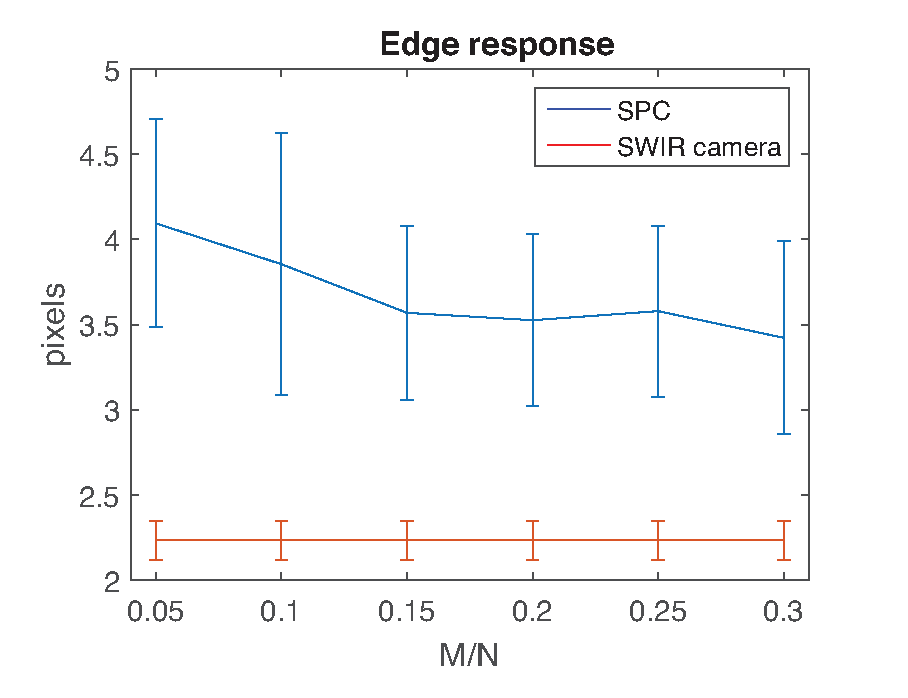
\includegraphics[width=0.7\linewidth]{result/mtf/Rise10_90.eps}
    \caption{10-90\% rise in pixels.}
    \label{fig:rise}
\end{figure}


\subsection{Luminance change in scene}
As predicted in section~\ref{sec:Dynamics_in_scene} dynamics in the scene could result in poor reconstruction performance.  

\subsection{Noise analysis}
Volt to variance
